\documentclass[border=3pt,tikz]{standalone}
\usepackage{amsmath}
\usetikzlibrary{3d} 
\usetikzlibrary{arrows}
\usetikzlibrary{shapes.geometric}
\begin{document}
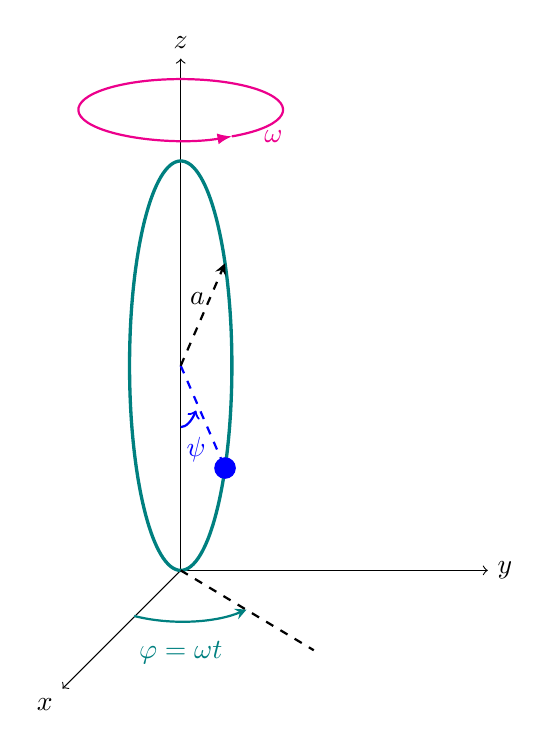
\begin{tikzpicture}[scale = 1.3, =>stealth]
    \tikzset{
        partial ellipse/.style args={#1:#2:#3}{
            insert path={+ (#1:#3) arc (#1:#2:#3)}
        }
    }
    \draw [->] (0,0) -- (xyz cs:x=3) node[right] {$y$};
    \draw [->] (0,0) -- (xyz cs:y=5) node [above] {$z$};
    \draw [->] (0,0) -- (xyz cs:z=3) node [below left] {$x$}; 
    \draw [very thick, teal] (0.0,2) ellipse (0.5 and 2);
      
    \draw [-latex, thick, magenta] (xyz cs:x=0.5, y=4.24) arc [start angle=300, end angle=660, x radius=1cm, y radius=0.3cm] node [xshift=15] {$\omega$};
    %   \draw [thick, -{stealth}] (0, 0) -- (xyz cs:x=0.7,y=2.55);
    %   \node[below, scale=.6] at (0.3, 2.3) {$\boldsymbol{r}_i (q_j)$};
    %   \draw [thick, -{stealth}] (0, 0) --(xyz cs:x=1.4,y=2.8);
    %   \node[scale=.6] at (1.5, 1.7) {$\boldsymbol{r}_i (q_j+dq_j)$};
    %   \draw [red, thick, -{stealth}] (0.7, 2.55) -- (1.4, 2.8);
    %   \node[red, scale=.6] at (1.0, 2.5) {$d\boldsymbol{r}_i$};
    %   \draw [thick, -{stealth}] (0, 3) -- (0, 3.7) node[right, scale=0.6] {$\;\hat{\boldsymbol{n}}$};
    
    \filldraw [blue] (xyz cs:x=0.4330, y=1) circle [radius=0.1];
    \draw [blue, thick, dashed] (0, 2) -- (0.4330, 1);
    \draw [->, thick, blue] (xyz cs:x=0, y=1.4) arc [start angle=270, end angle=300, x radius=0.3cm, y radius=1.2cm] node [below,yshift=-6] {$\psi$};    
    \draw [black, thick, dashed, -{stealth}] (0, 2) --node[above, xshift=-2] {$a$} (0.4330, 3);


    \draw[thick, teal, -{stealth}] (xyz cs:x=0, y=0) [partial ellipse=243:310:1. and 0.5] ;
    \node at (0.0, -0.6) [teal, below] {$\varphi =\omega t$};
    \draw[thick, dashed] (0, 0) -- ({1*1.3}, -{0.6*1.3});


\end{tikzpicture}
\end{document}